\documentclass[twoside]{book}

% Packages required by doxygen
\usepackage{fixltx2e}
\usepackage{calc}
\usepackage{doxygen}
\usepackage[export]{adjustbox} % also loads graphicx
\usepackage{graphicx}
\usepackage[utf8]{inputenc}
\usepackage{makeidx}
\usepackage{multicol}
\usepackage{multirow}
\PassOptionsToPackage{warn}{textcomp}
\usepackage{textcomp}
\usepackage[nointegrals]{wasysym}
\usepackage[table]{xcolor}

% Font selection
\usepackage[T1]{fontenc}
\usepackage[scaled=.90]{helvet}
\usepackage{courier}
\usepackage{amssymb}
\usepackage{sectsty}
\renewcommand{\familydefault}{\sfdefault}
\allsectionsfont{%
  \fontseries{bc}\selectfont%
  \color{darkgray}%
}
\renewcommand{\DoxyLabelFont}{%
  \fontseries{bc}\selectfont%
  \color{darkgray}%
}
\newcommand{\+}{\discretionary{\mbox{\scriptsize$\hookleftarrow$}}{}{}}

% Page & text layout
\usepackage{geometry}
\geometry{%
  a4paper,%
  top=2.5cm,%
  bottom=2.5cm,%
  left=2.5cm,%
  right=2.5cm%
}
\tolerance=750
\hfuzz=15pt
\hbadness=750
\setlength{\emergencystretch}{15pt}
\setlength{\parindent}{0cm}
\setlength{\parskip}{3ex plus 2ex minus 2ex}
\makeatletter
\renewcommand{\paragraph}{%
  \@startsection{paragraph}{4}{0ex}{-1.0ex}{1.0ex}{%
    \normalfont\normalsize\bfseries\SS@parafont%
  }%
}
\renewcommand{\subparagraph}{%
  \@startsection{subparagraph}{5}{0ex}{-1.0ex}{1.0ex}{%
    \normalfont\normalsize\bfseries\SS@subparafont%
  }%
}
\makeatother

% Headers & footers
\usepackage{fancyhdr}
\pagestyle{fancyplain}
\fancyhead[LE]{\fancyplain{}{\bfseries\thepage}}
\fancyhead[CE]{\fancyplain{}{}}
\fancyhead[RE]{\fancyplain{}{\bfseries\leftmark}}
\fancyhead[LO]{\fancyplain{}{\bfseries\rightmark}}
\fancyhead[CO]{\fancyplain{}{}}
\fancyhead[RO]{\fancyplain{}{\bfseries\thepage}}
\fancyfoot[LE]{\fancyplain{}{}}
\fancyfoot[CE]{\fancyplain{}{}}
\fancyfoot[RE]{\fancyplain{}{\bfseries\scriptsize Generated by Doxygen }}
\fancyfoot[LO]{\fancyplain{}{\bfseries\scriptsize Generated by Doxygen }}
\fancyfoot[CO]{\fancyplain{}{}}
\fancyfoot[RO]{\fancyplain{}{}}
\renewcommand{\footrulewidth}{0.4pt}
\renewcommand{\chaptermark}[1]{%
  \markboth{#1}{}%
}
\renewcommand{\sectionmark}[1]{%
  \markright{\thesection\ #1}%
}

% Indices & bibliography
\usepackage{natbib}
\usepackage[titles]{tocloft}
\setcounter{tocdepth}{3}
\setcounter{secnumdepth}{5}
\makeindex

% Hyperlinks (required, but should be loaded last)
\usepackage{ifpdf}
\ifpdf
  \usepackage[pdftex,pagebackref=true]{hyperref}
\else
  \usepackage[ps2pdf,pagebackref=true]{hyperref}
\fi
\hypersetup{%
  colorlinks=true,%
  linkcolor=blue,%
  citecolor=blue,%
  unicode%
}

% Custom commands
\newcommand{\clearemptydoublepage}{%
  \newpage{\pagestyle{empty}\cleardoublepage}%
}

\usepackage{caption}
\captionsetup{labelsep=space,justification=centering,font={bf},singlelinecheck=off,skip=4pt,position=top}

%===== C O N T E N T S =====

\begin{document}

% Titlepage & ToC
\hypersetup{pageanchor=false,
             bookmarksnumbered=true,
             pdfencoding=unicode
            }
\pagenumbering{alph}
\begin{titlepage}
\vspace*{7cm}
\begin{center}%
{\Large My Project }\\
\vspace*{1cm}
{\large Generated by Doxygen 1.8.14}\\
\end{center}
\end{titlepage}
\clearemptydoublepage
\pagenumbering{roman}
\tableofcontents
\clearemptydoublepage
\pagenumbering{arabic}
\hypersetup{pageanchor=true}

%--- Begin generated contents ---
\chapter{Hierarchical Index}
\section{Class Hierarchy}
This inheritance list is sorted roughly, but not completely, alphabetically\+:\begin{DoxyCompactList}
\item Stream\begin{DoxyCompactList}
\item \contentsline{section}{Esp\+Server}{\pageref{class_esp_server}}{}
\end{DoxyCompactList}
\end{DoxyCompactList}

\chapter{Data Structure Index}
\section{Data Structures}
Here are the data structures with brief descriptions\+:\begin{DoxyCompactList}
\item\contentsline{section}{\mbox{\hyperlink{class_esp_server}{Esp\+Server}} }{\pageref{class_esp_server}}{}
\end{DoxyCompactList}

\chapter{File Index}
\section{File List}
Here is a list of all documented files with brief descriptions\+:\begin{DoxyCompactList}
\item\contentsline{section}{\mbox{\hyperlink{_arduinopart_8ino}{Arduinopart.\+ino}} }{\pageref{_arduinopart_8ino}}{}
\item\contentsline{section}{{\bfseries Dumb\+Server.\+h} }{\pageref{_dumb_server_8h}}{}
\end{DoxyCompactList}

\chapter{Data Structure Documentation}
\hypertarget{class_esp_server}{}\section{Esp\+Server Class Reference}
\label{class_esp_server}\index{Esp\+Server@{Esp\+Server}}


Inheritance diagram for Esp\+Server\+:\nopagebreak
\begin{figure}[H]
\begin{center}
\leavevmode
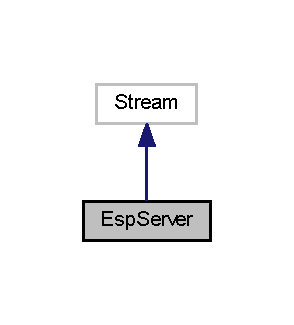
\includegraphics[width=141pt]{class_esp_server__inherit__graph}
\end{center}
\end{figure}


Collaboration diagram for Esp\+Server\+:\nopagebreak
\begin{figure}[H]
\begin{center}
\leavevmode
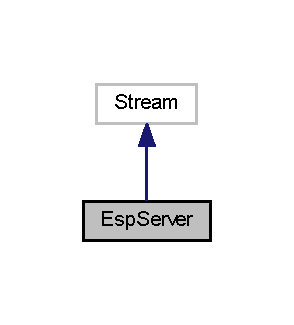
\includegraphics[width=141pt]{class_esp_server__coll__graph}
\end{center}
\end{figure}
\subsection*{Public Member Functions}
\begin{DoxyCompactItemize}
\item 
\mbox{\Hypertarget{class_esp_server_a1d8682ca0934af03639311e23a71283f}\label{class_esp_server_a1d8682ca0934af03639311e23a71283f}} 
void {\bfseries begin} (Stream $\ast$\mbox{\hyperlink{_arduinopart_8ino_af690b3a6882292855c4091ede8039998}{esp\+\_\+serial}}, const char $\ast$ssid, const char $\ast$pass, uint16\+\_\+t port)
\item 
\mbox{\Hypertarget{class_esp_server_a01953c4cc039c37f94dc3e1057126abb}\label{class_esp_server_a01953c4cc039c37f94dc3e1057126abb}} 
void {\bfseries my\+\_\+ip} (char $\ast$buf, size\+\_\+t buflen)
\item 
\mbox{\Hypertarget{class_esp_server_a59fc494d53391b27e2fd75cb750690d9}\label{class_esp_server_a59fc494d53391b27e2fd75cb750690d9}} 
bool {\bfseries connected} ()
\item 
\mbox{\Hypertarget{class_esp_server_a4549a76725f2e4c013e4d57018366109}\label{class_esp_server_a4549a76725f2e4c013e4d57018366109}} 
virtual int {\bfseries available} ()
\item 
\mbox{\Hypertarget{class_esp_server_a9040fa1d479d71edf3a826f4691c35c4}\label{class_esp_server_a9040fa1d479d71edf3a826f4691c35c4}} 
virtual int {\bfseries peek} ()
\item 
\mbox{\Hypertarget{class_esp_server_aaab5dab5b969a87f538242e524431637}\label{class_esp_server_aaab5dab5b969a87f538242e524431637}} 
virtual int {\bfseries read} ()
\item 
\mbox{\Hypertarget{class_esp_server_adac116554b543b7c4228c018a85882f5}\label{class_esp_server_adac116554b543b7c4228c018a85882f5}} 
virtual void {\bfseries flush} ()
\item 
\mbox{\Hypertarget{class_esp_server_a7c66fc8d559f4956d4ccea196299bca7}\label{class_esp_server_a7c66fc8d559f4956d4ccea196299bca7}} 
virtual size\+\_\+t {\bfseries write} (const uint8\+\_\+t $\ast$buffer, size\+\_\+t size)
\item 
\mbox{\Hypertarget{class_esp_server_af32c245c813bbadb566538bba418b0fe}\label{class_esp_server_af32c245c813bbadb566538bba418b0fe}} 
size\+\_\+t {\bfseries write} (uint8\+\_\+t n)
\item 
\mbox{\Hypertarget{class_esp_server_a0ba52a995edf9b6c2cdf3d396be84ff1}\label{class_esp_server_a0ba52a995edf9b6c2cdf3d396be84ff1}} 
size\+\_\+t {\bfseries write} (unsigned long n)
\item 
\mbox{\Hypertarget{class_esp_server_a3cfec102ee6f58a2f7e617999ce9f5bb}\label{class_esp_server_a3cfec102ee6f58a2f7e617999ce9f5bb}} 
size\+\_\+t {\bfseries write} (long n)
\item 
\mbox{\Hypertarget{class_esp_server_a2d9bc6ac05e45a7023be3cd1ca224407}\label{class_esp_server_a2d9bc6ac05e45a7023be3cd1ca224407}} 
size\+\_\+t {\bfseries write} (unsigned int n)
\item 
\mbox{\Hypertarget{class_esp_server_a22e7ab55e0aa268cff5b48e763429ec3}\label{class_esp_server_a22e7ab55e0aa268cff5b48e763429ec3}} 
size\+\_\+t {\bfseries write} (int n)
\end{DoxyCompactItemize}


The documentation for this class was generated from the following files\+:\begin{DoxyCompactItemize}
\item 
Dumb\+Server.\+h\item 
Dumb\+Server.\+cpp\end{DoxyCompactItemize}

\chapter{File Documentation}
\hypertarget{_arduinopart_8ino}{}\section{Arduinopart.\+ino File Reference}
\label{_arduinopart_8ino}\index{Arduinopart.\+ino@{Arduinopart.\+ino}}
{\ttfamily \#include $<$Servo.\+h$>$}\newline
{\ttfamily \#include \char`\"{}Dumb\+Server.\+h\char`\"{}}\newline
{\ttfamily \#include $<$Software\+Serial.\+h$>$}\newline
Include dependency graph for Arduinopart.\+ino\+:\nopagebreak
\begin{figure}[H]
\begin{center}
\leavevmode
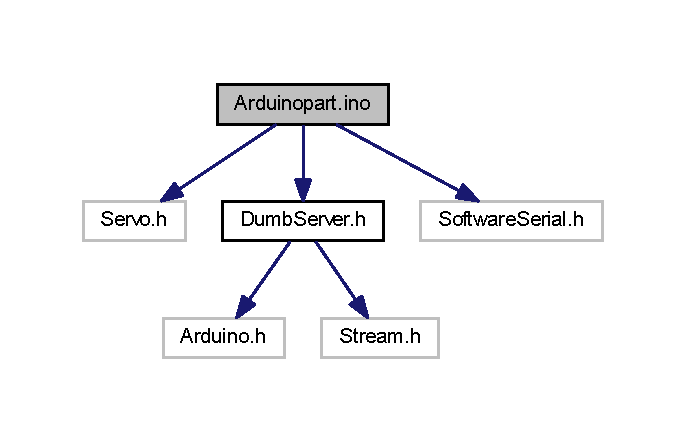
\includegraphics[width=329pt]{_arduinopart_8ino__incl}
\end{center}
\end{figure}
\subsection*{Functions}
\begin{DoxyCompactItemize}
\item 
Software\+Serial \mbox{\hyperlink{_arduinopart_8ino_af690b3a6882292855c4091ede8039998}{esp\+\_\+serial}} (3, 2)
\item 
void \mbox{\hyperlink{_arduinopart_8ino_a4fc01d736fe50cf5b977f755b675f11d}{setup}} ()
\item 
void \mbox{\hyperlink{_arduinopart_8ino_afe461d27b9c48d5921c00d521181f12f}{loop}} ()
\end{DoxyCompactItemize}
\subsection*{Variables}
\begin{DoxyCompactItemize}
\item 
\mbox{\Hypertarget{_arduinopart_8ino_a92309e3a6d185d9188757bac49168fe5}\label{_arduinopart_8ino_a92309e3a6d185d9188757bac49168fe5}} 
\mbox{\hyperlink{class_esp_server}{Esp\+Server}} {\bfseries esp\+\_\+server}
\item 
Servo \mbox{\hyperlink{_arduinopart_8ino_ac5d2bea44c6318454db0e2639a4efe95}{servo1}}
\item 
int \mbox{\hyperlink{_arduinopart_8ino_a774b9921c97f68fcf97c8c5b41cef667}{servo\+Pin1}} = 9
\item 
int \mbox{\hyperlink{_arduinopart_8ino_af3a750927bb0dac8a337245b7d570a6d}{Zaehler}} = 0
\item 
int \mbox{\hyperlink{_arduinopart_8ino_acb85827c057a298dc883f002985f7abf}{in\+Pin1}} = 11
\item 
int \mbox{\hyperlink{_arduinopart_8ino_a948167f8090ebc248e42325a827e9371}{val1}} = 0
\item 
int \mbox{\hyperlink{_arduinopart_8ino_acc3748d7169a359b540e60b40b6a8956}{val2}} = 0
\item 
int \mbox{\hyperlink{_arduinopart_8ino_ae94f1e0f6ff148a9f305e17a2c2894fb}{servo\+Angle1}} = 0
\item 
int \mbox{\hyperlink{_arduinopart_8ino_abc65d3b1e9a28ec21cbb4b1d23b77d10}{in\+Pin2}} = 13
\item 
int \mbox{\hyperlink{_arduinopart_8ino_a8c935df72ad1a7236c9879fb14aa0d43}{led}} = 12
\end{DoxyCompactItemize}


\subsection{Function Documentation}
\mbox{\Hypertarget{_arduinopart_8ino_af690b3a6882292855c4091ede8039998}\label{_arduinopart_8ino_af690b3a6882292855c4091ede8039998}} 
\index{Arduinopart.\+ino@{Arduinopart.\+ino}!esp\+\_\+serial@{esp\+\_\+serial}}
\index{esp\+\_\+serial@{esp\+\_\+serial}!Arduinopart.\+ino@{Arduinopart.\+ino}}
\subsubsection{\texorpdfstring{esp\+\_\+serial()}{esp\_serial()}}
{\footnotesize\ttfamily Software\+Serial esp\+\_\+serial (\begin{DoxyParamCaption}\item[{3}]{,  }\item[{2}]{ }\end{DoxyParamCaption})}

The Wifi shield is connected to the Arduino-\/\+Pins 2 and 3 Here is the caller graph for this function\+:\nopagebreak
\begin{figure}[H]
\begin{center}
\leavevmode
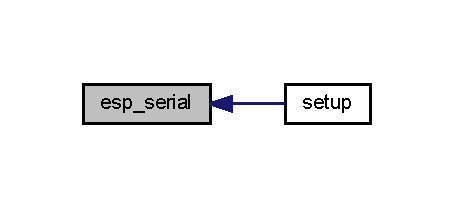
\includegraphics[width=218pt]{_arduinopart_8ino_af690b3a6882292855c4091ede8039998_icgraph}
\end{center}
\end{figure}
\mbox{\Hypertarget{_arduinopart_8ino_afe461d27b9c48d5921c00d521181f12f}\label{_arduinopart_8ino_afe461d27b9c48d5921c00d521181f12f}} 
\index{Arduinopart.\+ino@{Arduinopart.\+ino}!loop@{loop}}
\index{loop@{loop}!Arduinopart.\+ino@{Arduinopart.\+ino}}
\subsubsection{\texorpdfstring{loop()}{loop()}}
{\footnotesize\ttfamily void loop (\begin{DoxyParamCaption}{ }\end{DoxyParamCaption})}

say y to the client ~\newline
 say n to the client \mbox{\Hypertarget{_arduinopart_8ino_a4fc01d736fe50cf5b977f755b675f11d}\label{_arduinopart_8ino_a4fc01d736fe50cf5b977f755b675f11d}} 
\index{Arduinopart.\+ino@{Arduinopart.\+ino}!setup@{setup}}
\index{setup@{setup}!Arduinopart.\+ino@{Arduinopart.\+ino}}
\subsubsection{\texorpdfstring{setup()}{setup()}}
{\footnotesize\ttfamily void setup (\begin{DoxyParamCaption}{ }\end{DoxyParamCaption})}

$<$send to the Client on 9600 Baud$>$ ~\newline
~\newline
~\newline
~\newline
~\newline
~\newline
~\newline
 $<$send to the Serial\+Port on 9600 Baud$>$ ~\newline
~\newline
~\newline
~\newline
~\newline
~\newline
 $<$ declare Servo\+Pin1 as a Servopin for the Library ~\newline
~\newline
~\newline
~\newline
~\newline
 $<$ set the poristion of the Servo\+Pin to 0 ~\newline
~\newline
~\newline
~\newline
 declare pushbutton as input ~\newline
~\newline
~\newline
 declare pushbutton 2 as input ~\newline
~\newline
 declare L\+ED as Output ~\newline
 Get and print the I\+P-\/\+Address to which the Python should connect to Here is the call graph for this function\+:\nopagebreak
\begin{figure}[H]
\begin{center}
\leavevmode
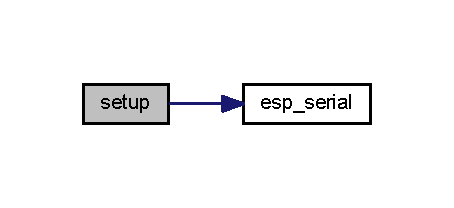
\includegraphics[width=218pt]{_arduinopart_8ino_a4fc01d736fe50cf5b977f755b675f11d_cgraph}
\end{center}
\end{figure}


\subsection{Variable Documentation}
\mbox{\Hypertarget{_arduinopart_8ino_acb85827c057a298dc883f002985f7abf}\label{_arduinopart_8ino_acb85827c057a298dc883f002985f7abf}} 
\index{Arduinopart.\+ino@{Arduinopart.\+ino}!in\+Pin1@{in\+Pin1}}
\index{in\+Pin1@{in\+Pin1}!Arduinopart.\+ino@{Arduinopart.\+ino}}
\subsubsection{\texorpdfstring{in\+Pin1}{inPin1}}
{\footnotesize\ttfamily int in\+Pin1 = 11}

define the Pin 11 for the 1. Pushbutton \mbox{\Hypertarget{_arduinopart_8ino_abc65d3b1e9a28ec21cbb4b1d23b77d10}\label{_arduinopart_8ino_abc65d3b1e9a28ec21cbb4b1d23b77d10}} 
\index{Arduinopart.\+ino@{Arduinopart.\+ino}!in\+Pin2@{in\+Pin2}}
\index{in\+Pin2@{in\+Pin2}!Arduinopart.\+ino@{Arduinopart.\+ino}}
\subsubsection{\texorpdfstring{in\+Pin2}{inPin2}}
{\footnotesize\ttfamily int in\+Pin2 = 13}

define the Pin 13 for the Pushbutton 2 \mbox{\Hypertarget{_arduinopart_8ino_a8c935df72ad1a7236c9879fb14aa0d43}\label{_arduinopart_8ino_a8c935df72ad1a7236c9879fb14aa0d43}} 
\index{Arduinopart.\+ino@{Arduinopart.\+ino}!led@{led}}
\index{led@{led}!Arduinopart.\+ino@{Arduinopart.\+ino}}
\subsubsection{\texorpdfstring{led}{led}}
{\footnotesize\ttfamily int led = 12}

define the Pin 12 for the L\+ED $>$ \mbox{\Hypertarget{_arduinopart_8ino_ac5d2bea44c6318454db0e2639a4efe95}\label{_arduinopart_8ino_ac5d2bea44c6318454db0e2639a4efe95}} 
\index{Arduinopart.\+ino@{Arduinopart.\+ino}!servo1@{servo1}}
\index{servo1@{servo1}!Arduinopart.\+ino@{Arduinopart.\+ino}}
\subsubsection{\texorpdfstring{servo1}{servo1}}
{\footnotesize\ttfamily Servo servo1}

define servo1 as a Servo for the servo library \mbox{\Hypertarget{_arduinopart_8ino_ae94f1e0f6ff148a9f305e17a2c2894fb}\label{_arduinopart_8ino_ae94f1e0f6ff148a9f305e17a2c2894fb}} 
\index{Arduinopart.\+ino@{Arduinopart.\+ino}!servo\+Angle1@{servo\+Angle1}}
\index{servo\+Angle1@{servo\+Angle1}!Arduinopart.\+ino@{Arduinopart.\+ino}}
\subsubsection{\texorpdfstring{servo\+Angle1}{servoAngle1}}
{\footnotesize\ttfamily int servo\+Angle1 = 0}

define the servo\+Angle as 0 as starting Angle \mbox{\Hypertarget{_arduinopart_8ino_a774b9921c97f68fcf97c8c5b41cef667}\label{_arduinopart_8ino_a774b9921c97f68fcf97c8c5b41cef667}} 
\index{Arduinopart.\+ino@{Arduinopart.\+ino}!servo\+Pin1@{servo\+Pin1}}
\index{servo\+Pin1@{servo\+Pin1}!Arduinopart.\+ino@{Arduinopart.\+ino}}
\subsubsection{\texorpdfstring{servo\+Pin1}{servoPin1}}
{\footnotesize\ttfamily int servo\+Pin1 = 9}

define Pin 9 as the Servo Pin \mbox{\Hypertarget{_arduinopart_8ino_a948167f8090ebc248e42325a827e9371}\label{_arduinopart_8ino_a948167f8090ebc248e42325a827e9371}} 
\index{Arduinopart.\+ino@{Arduinopart.\+ino}!val1@{val1}}
\index{val1@{val1}!Arduinopart.\+ino@{Arduinopart.\+ino}}
\subsubsection{\texorpdfstring{val1}{val1}}
{\footnotesize\ttfamily int val1 = 0}

define the val1 for the Pushbutton 1 \mbox{\Hypertarget{_arduinopart_8ino_acc3748d7169a359b540e60b40b6a8956}\label{_arduinopart_8ino_acc3748d7169a359b540e60b40b6a8956}} 
\index{Arduinopart.\+ino@{Arduinopart.\+ino}!val2@{val2}}
\index{val2@{val2}!Arduinopart.\+ino@{Arduinopart.\+ino}}
\subsubsection{\texorpdfstring{val2}{val2}}
{\footnotesize\ttfamily int val2 = 0}

define the val2 for the Pushbutton 2 \mbox{\Hypertarget{_arduinopart_8ino_af3a750927bb0dac8a337245b7d570a6d}\label{_arduinopart_8ino_af3a750927bb0dac8a337245b7d570a6d}} 
\index{Arduinopart.\+ino@{Arduinopart.\+ino}!Zaehler@{Zaehler}}
\index{Zaehler@{Zaehler}!Arduinopart.\+ino@{Arduinopart.\+ino}}
\subsubsection{\texorpdfstring{Zaehler}{Zaehler}}
{\footnotesize\ttfamily int Zaehler = 0}

define a Counter for how often the Mailbox has been opened 
%--- End generated contents ---

% Index
\backmatter
\newpage
\phantomsection
\clearemptydoublepage
\addcontentsline{toc}{chapter}{Index}
\printindex

\end{document}
